\documentclass{standalone}


\usepackage{fontspec}
\usepackage{sunpath}
\usetikzlibrary{hobby}

\usepackage{hyperref}

\pagecolor{white}
\begin{document}
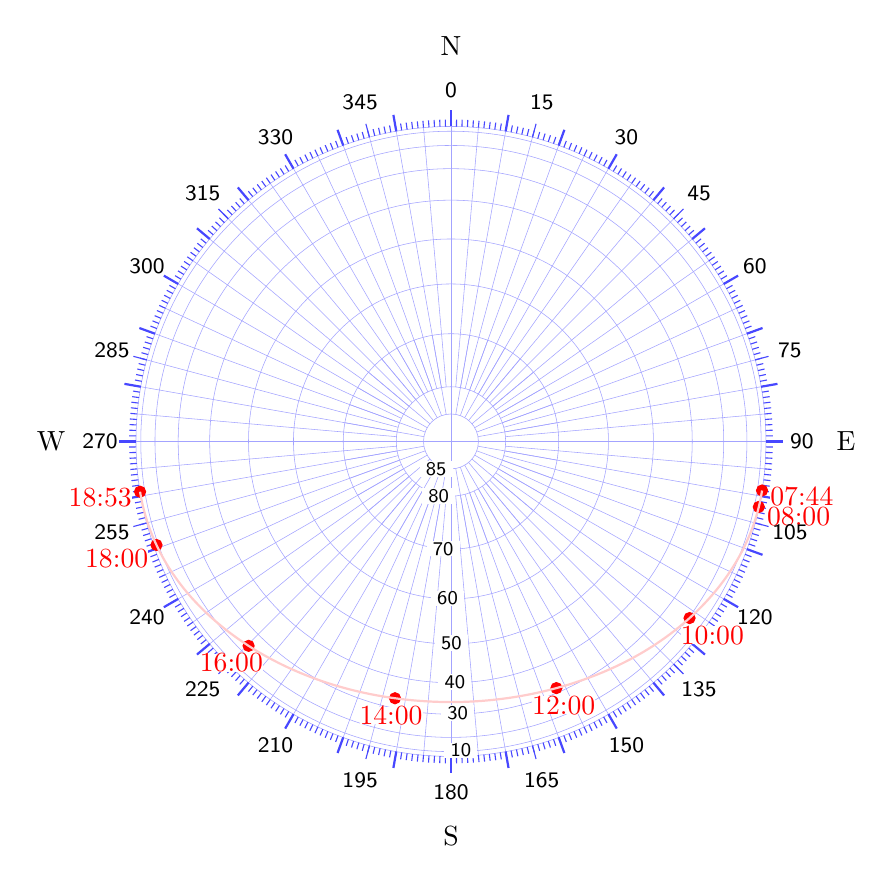
\begin{tikzpicture}[spradius=4]
\tikzset{
  sun path curve/.style={draw=red!20,thick},
  sun point/.style={radius=2pt,draw=red,fill=red},  
  sun label/.style={below,fill=white,outer sep=3pt,inner sep=0pt,text=red},
  small alt label/.style={altitude label,font=\scriptsize\sffamily}
}
\spcrosshair
\spaltitudecircle{{0,10,...,80,85}}
\spazimuthline{{0,10,...,360}}{85}{70}
\spazimuthline{{0,5,...,360}}{80}{0}
\spazimuthtick

\coordinate (P0) at (sunpath cs:azi=98.968673,alt=-0.208672);
\coordinate (P1) at (sunpath cs:azi=102.009695,alt=2.035492);
\coordinate (P2) at (sunpath cs:azi=126.513583,alt=19.499874);
\coordinate (P3) at (sunpath cs:azi=156.854847,alt=31.593335);
\coordinate (P4) at (sunpath cs:azi=192.292832,alt=33.425294);
\coordinate (P5) at (sunpath cs:azi=224.708002,alt=24.034984);
\coordinate (P6) at (sunpath cs:azi=250.626597,alt=7.619801);
\coordinate (P7) at (sunpath cs:azi=260.810553,alt=-0.244637);
\path[sun point] (P0) circle;
\path[sun point] (P1) circle;
\path[sun point] (P2) circle;
\path[sun point] (P3) circle;
\path[sun point] (P4) circle;
\path[sun point] (P5) circle;
\path[sun point] (P6) circle;
\path[sun point] (P7) circle;
\node[sun label,anchor=270-98.968673] at (P0) {07:44};
\node[sun label,anchor=270-102.009695] at (P1) {08:00};
\node[sun label,anchor=270-126.513583] at (P2) {10:00};
\node[sun label,anchor=270-156.854847] at (P3) {12:00};
\node[sun label,anchor=270-192.292832] at (P4) {14:00};
\node[sun label,anchor=270-224.708002] at (P5) {16:00};
\node[sun label,anchor=270-250.626597] at (P6) {18:00};
\node[sun label,anchor=270-260.810553] at (P7) {18:53};
\path[sun path curve] (P0) to [curve through={ (P1) .. (P2) .. (P3) .. (P4) .. (P5) .. (P6) }] (P7) ;

\spaltitudelabel{{10,30,40,...,80,85}}[175][small alt label]
\spazimuthlabel{{0,15,...,350}}
\spgeodirection
\end{tikzpicture}
\end{document}

